% ==============================================
% !TEX root = ./critics.tex
% ==============================================
% ==============================================
\section{Motivating Examples and Tool Features}
\label{sec:motivation}
% ==============================================
\begin{figure}
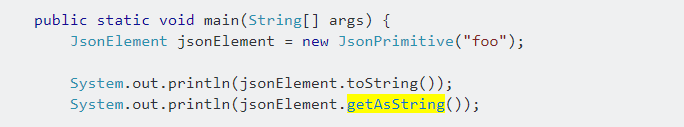
\includegraphics[width=0.48\textwidth]{json_ex1.PNG}
\vspace{.1in}
\caption{A code snippet that does not properly check {\tt JsonElement.getAsString}.\protect\footnotemark}
\label{fig:arch}
\end{figure}

\footnotetext{https://stackoverflow.com/questions/34120882/gson-jsonelement-getasstring-vs-jsonelement-tostring}

Consider Alice, a software developer who needs to develop a feature for a program using Google's Gson library for Java\footnote{https://github.com/google/gson/blob/master/UserGuide.md}, which she is unfamiliar with. Alice uses an Internet search engine to look up how to use Gson's {\tt JsonElement}'s {\tt getAsString()} method and finds a post on Stack Overflow, as shown in Figure 2. However, this example does not use the {\tt JsonElement} API completely correctly. 

{\bf Stack Overflow Post View.}
Alice is running Maple's Chrome extension when she finds this post, and the extension highlights the potential API misuse in the code snippet, as seen in Figure 2. Note that the extension only highlights the first instance of this misuse although it occurs multiple times in the code snippet, to eliminate redundancy and avoid confusion. Alice is interested in learning more about the API and what specifically the code snippet did not include, so she clicks on the highlighted text.

\begin{figure}
\centering
  \begin{subfigure}[a]{0.48\textwidth}
  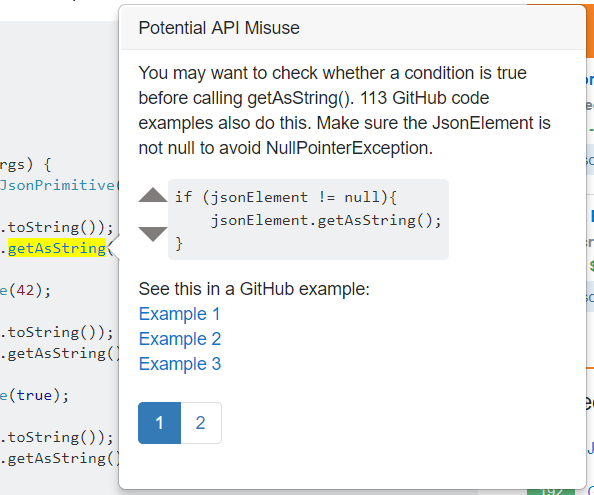
\includegraphics[width=\textwidth]{json_ex2.PNG}
  \caption{A page describing a way to avoid a {\tt ClassCastException} by checking whether the {\tt JsonElement} object is a primitive.} 
  \vspace{.1in}
  \label{fig:arch}
  \end{subfigure}
  \hfill
  \begin{subfigure}[b]{0.48\textwidth}
  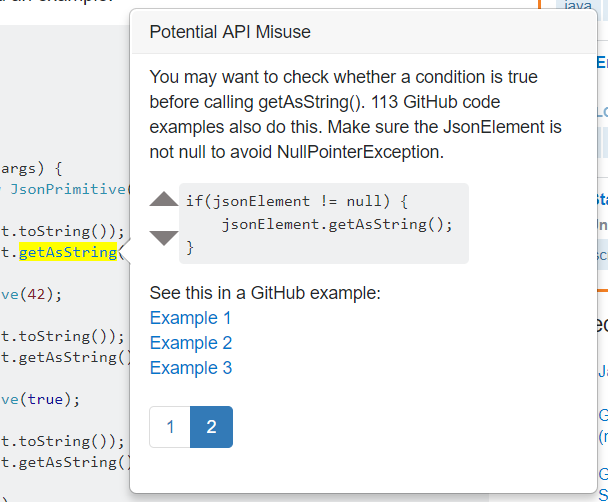
\includegraphics[width=\textwidth]{json_ex3.PNG}
  \caption{A page describing a way to avoid a {\tt NullPointerException} by checking whether the {\tt JsonElement} object is null.}
  \vspace{.1in}
  \label{fig:arch}
  \end{subfigure}
  \hfill
\caption{The two pages of a popup generated on {\tt JsonElement.getAsString}.}
\end{figure}

{\bf Stack Overflow Popup View.}
Clicking on the highlighted text reveals a popup, as seen in Figure 3. The popup is populated with information about any required patterns in Maple's database this particular API call does not adhere to. Alice notices that there are two pages of the popup, indicating two different usage patterns that this call does not follow, as shown in Figures 3a and 3b. 

Alice inspects the first page (Fig. 3a) and learns that she should check whether the {\tt JsonElement} object is a primitive before calling {\tt getAsString} in order to avoid a {\tt ClassCastException}. She notices that 52 other GitHub code examples use this pattern, which gives her a qualitative measurement of how prevalent this pattern is in compiled, "real world" code.
Alice then inspects the second page (Fig. 3b), and finds that it suggests a null check before calling {\tt getAsString}. She notices that this pattern has more than double the support of the previous pattern.

Curious to see the first pattern in context, Alice returns to the first page of the popup and clicks on the first link provided to her under "See this in a GitHub example."

\begin{figure}
\centering
  \begin{subfigure}[a]{0.48\textwidth}
  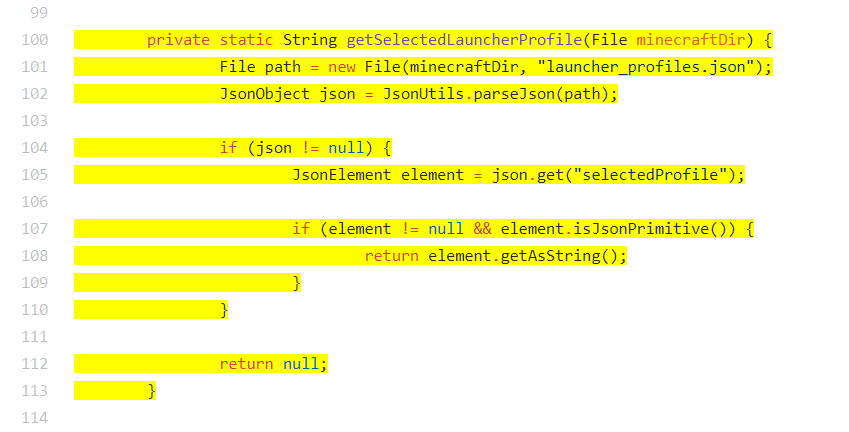
\includegraphics[width=\textwidth]{json_primitive_gh1.PNG}
  \caption{The first GitHub example for Figure 3a.} 
  \vspace{.1in}
  \label{fig:arch}
  \end{subfigure}
  \hfill
  \begin{subfigure}[b]{0.48\textwidth}
  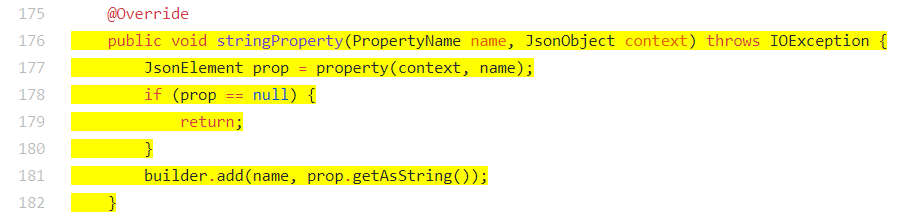
\includegraphics[width=\textwidth]{json_null_gh2.PNG}
  \caption{The second GitHub example for Figure 3b.}
  \vspace{.1in}
  \label{fig:arch}
  \end{subfigure}
  \hfill
\caption{The highlighted GitHub examples redirected to from the links provided in the popup.}
\end{figure}

{\bf GitHub Example View.} When Alice clicks on one of the GitHub links, the file opens in a new tab and the view scrolls to where the API is called in the file, and the method in which this occurs is highlighted so Alice can easily find it, as seen in Figure 4. The addition of a compilable code example that demonstrates the pattern in context can aid Alice in understanding how to use the pattern if it is unfamiliar to her. In this case, Alice finds herself redirected the method in a GitHub project seen in Figure 4a. She notices that the example uses a null check in conjunction with the primitive check, which makes sense to her after seeing that both were missing from the Stack Overflow code snippet.

Returning to the popup in Stack Overflow, Alice clicks on the second link provided for the second page to compare usage patterns in context. This link opens up to the GitHub method seen in Figure 4b. Unlike the one in Figure 4a, this example does not use the null check in conjunction with the primitive check. 

After seeing these two examples, Alice can infer that a null check is more necessary and is more common than the primitive check, based on the GitHub examples she has seen as well as the GitHub support indicated by the popup message. She upvotes the null check's pattern by clicking on the up-arrow on its page (see Figure 3b) to send the server her feedback on the patterns it gave her. 

